%!TEX root = ../effc_top.tex

\begin{frame}{Operations at odd primes}

	\pause

	Steenrod squares come from making a \textbf{binary} coproduct $C \to C^{\ot 2}$ cocommutative up to coherent homotopies.

	\medskip\pause

	Steenrod also defined operations (for $\beta \in \{0,1\}$)
	\[
	\beta^{\varepsilon} P_k \colon H^\bullet(X; \Fp) \to H^\bullet(X; \Fp).
	\]

	\pause

	They come from making a coproduct $C \to C^{\ot p}$ commutative up to coherent homotopies.

	\medskip\pause

	A coherent structure controlling these is that of an $E_\infty$-coalgebra.

	\medskip\pause

	$E_\infty$-structures have a long history:
	\begin{itemize}
		\item (co)homology operations,
		\item recognition of infinite loop spaces,
		\item algebraic representation of the $p$-adic homotopy category.
	\end{itemize}

	\medskip\pause

	Defined using framework of operads.
\end{frame}

\begin{frame}{An $E_\infty$-coalgebra on chains}
	\begin{theorem}[Med.]
		The collection of maps $\gchains(\gsimplex^n) \to \gchains(\gsimplex^n)^{\otimes r}$ obtained from compositions of
		\begin{align*}
			\Delta &\colon \gchains(\gsimplex^n) \to \gchains(\gsimplex^n)^{\otimes 2}
			\qquad \text{(AW diagonal)} \\
			\ast &\colon \gchains(\gsimplex^n)^{\otimes 2} \to \gchains(\gsimplex^n)
			\qquad \text{(Join map)}
		\end{align*}
		defines an $E_\infty$-coalgebra on simplicial chains.
	\end{theorem}

	\pause

	\qquad \qquad \scalebox{0.7}{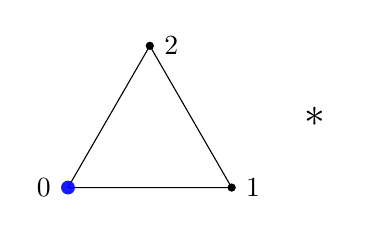
\begin{tikzpicture}[scale=.6]
\coordinate (A) at (210:2);
\coordinate (B) at (-30:2);
\coordinate (C) at (90:2);

\draw[draw=black] (A) -- (B) -- (C) -- (A);

\node[circle,fill=blue, opacity=.9, inner sep=0pt,minimum size=5pt, label=left:{0}] (a) at (A) {};
\node[circle,fill=black,inner sep=0pt,minimum size=3pt, label=right:{$1$}] (a) at (B) {};
\node[circle,fill=black,inner sep=0pt,minimum size=3pt, label=right:{$2$}] (a) at (C) {};

\node[scale=1.5] at (3.5,0.5) {$\ast$};
\end{tikzpicture}
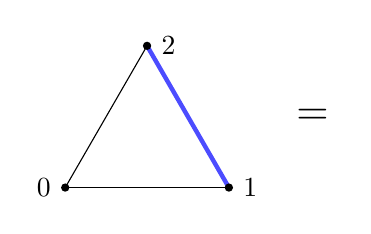
\begin{tikzpicture}[scale=.6]
\coordinate (A) at (210:2);
\coordinate (B) at (-30:2);
\coordinate (C) at (90:2);

\draw[draw=blue,  ultra thick, draw opacity=.7] (B) -- (C);
\draw[draw=black] (C) -- (A);
\draw[draw=black] (A) -- (B);

\node[circle,fill=black,inner sep=0pt,minimum size=3pt, label=left:{$0$}] (a) at (A) {};
\node[circle,fill=black,inner sep=0pt,minimum size=3pt, label=right:{$1$}] (a) at (B) {};
\node[circle,fill=black,inner sep=0pt,minimum size=3pt, label=right:{$2$}] (a) at (C) {};

\node[scale=1.5] at (3.5,.5) {=};
\end{tikzpicture}
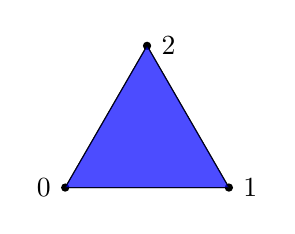
\begin{tikzpicture}[scale=.6]
\coordinate (A) at (210:2);
\coordinate (B) at (-30:2);
\coordinate (C) at (90:2);

\draw[draw=black] (A) -- (B) -- (C) -- (A);

\node[circle,fill=black,inner sep=0pt,minimum size=3pt, label=left:{$0$}] (a) at (A) {};
\node[circle,fill=black,inner sep=0pt,minimum size=3pt, label=right:{$1$}] (a) at (B) {};
\node[circle,fill=black,inner sep=0pt,minimum size=3pt, label=right:{$2$}] (a) at (C) {};

\draw[draw, fill=blue, opacity=.7] (A) -- (B) -- (C) -- (A);
\end{tikzpicture}}

	\medskip\pause

	Also, versions for: \par
		\qquad \textcolor{pblue}{cubical} (Kaufmann--Med.) and \par
		\qquad \textcolor{pblue}{multisimplicial} (Med.--Pizzi--Salvatore) chains.

%	\pause Furthermore, the assignments
%	\[
%	\coproduct \mapsto \Delta
%	\qquad
%	\product \mapsto \ast
%	\vspace*{-10pt}
%	\]
%	where
%	\[
%	\Delta \colon \gchains(\gsimplex^n) \to \gchains(\gsimplex^n)^{\otimes 2}, \qquad
%	\ast \colon \gchains(\gsimplex^n)^{\otimes 2} \to \gchains(\gsimplex^n)
%	\]
%	are the AW coproduct and the algebraic join, \pause
%	and in the cubical case the CS coproduct and a suitable analogue, induce the following.
%	\pause
%	\begin{theorem}[Med.]
%		The complexes $\gchains(\gsimplex^n)$ and $\gchains(\gcube^n)$ are natural $\UMed$-coalgebras.
%	\end{theorem}
%	\pause
%	We remark that explicitly describable elements in $\UMed(2)$ recover the Steenrod cup-$i$ coproducts in the simplicial and cubical case.
\end{frame}

%\begin{frame}[t]{Beyond the even prime}
%
%	\pause
%
%	Extending the diagonal to a full \textcolor{pblue}{$E_\infty$-coalgebra} structure on chains.
%
%	\smallskip\pause
%
%	These provide an algebraic model for the homotopy theory of spaces.\\ e.g. over $\mathbb Q$ (Quillen--Sullivan) over $\overline{\mathbb F}_p$ (Mandell).
%
%	\smallskip\pause
%
%	\begin{theorem}[Med.]
%		The collection of maps $\gchains(\gsimplex^n) \to \gchains(\gsimplex^n)^{\otimes r}$ obtained from compositions of
%		\begin{align*}
%		\Delta &\colon \gchains(\gsimplex^n) \to \gchains(\gsimplex^n)^{\otimes 2}
%		\qquad \text{(AW diagonal)} \\
%		\ast &\colon \gchains(\gsimplex^n)^{\otimes 2} \to \gchains(\gsimplex^n)
%		\qquad \text{(Join map)}
%		\end{align*}
%		defines an $E_\infty$-coalgebra on simplicial chains.
%	\end{theorem}
%
%	\pause
%
%	\only<5>{\qquad \qquad \scalebox{0.7}{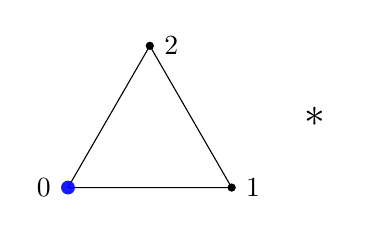
\begin{tikzpicture}[scale=.6]
\coordinate (A) at (210:2);
\coordinate (B) at (-30:2);
\coordinate (C) at (90:2);

\draw[draw=black] (A) -- (B) -- (C) -- (A);

\node[circle,fill=blue, opacity=.9, inner sep=0pt,minimum size=5pt, label=left:{0}] (a) at (A) {};
\node[circle,fill=black,inner sep=0pt,minimum size=3pt, label=right:{$1$}] (a) at (B) {};
\node[circle,fill=black,inner sep=0pt,minimum size=3pt, label=right:{$2$}] (a) at (C) {};

\node[scale=1.5] at (3.5,0.5) {$\ast$};
\end{tikzpicture}
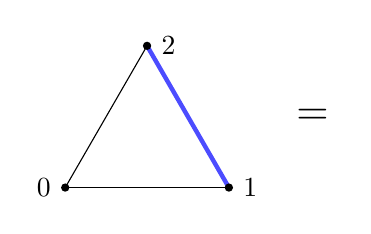
\begin{tikzpicture}[scale=.6]
\coordinate (A) at (210:2);
\coordinate (B) at (-30:2);
\coordinate (C) at (90:2);

\draw[draw=blue,  ultra thick, draw opacity=.7] (B) -- (C);
\draw[draw=black] (C) -- (A);
\draw[draw=black] (A) -- (B);

\node[circle,fill=black,inner sep=0pt,minimum size=3pt, label=left:{$0$}] (a) at (A) {};
\node[circle,fill=black,inner sep=0pt,minimum size=3pt, label=right:{$1$}] (a) at (B) {};
\node[circle,fill=black,inner sep=0pt,minimum size=3pt, label=right:{$2$}] (a) at (C) {};

\node[scale=1.5] at (3.5,.5) {=};
\end{tikzpicture}
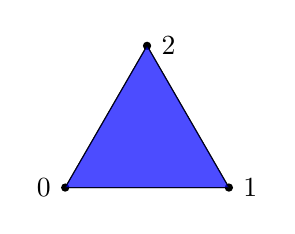
\begin{tikzpicture}[scale=.6]
\coordinate (A) at (210:2);
\coordinate (B) at (-30:2);
\coordinate (C) at (90:2);

\draw[draw=black] (A) -- (B) -- (C) -- (A);

\node[circle,fill=black,inner sep=0pt,minimum size=3pt, label=left:{$0$}] (a) at (A) {};
\node[circle,fill=black,inner sep=0pt,minimum size=3pt, label=right:{$1$}] (a) at (B) {};
\node[circle,fill=black,inner sep=0pt,minimum size=3pt, label=right:{$2$}] (a) at (C) {};

\draw[draw, fill=blue, opacity=.7] (A) -- (B) -- (C) -- (A);
\end{tikzpicture}}}
%
%	\medskip\pause
%
%	\only<6>{Also, versions for: \par
%		\qquad \textcolor{pblue}{cubical} (Kaufmann--Med.) and \par
%		\qquad \textcolor{pblue}{multisimplicial} (Med.--Pizzi--Salvatore) chains.}
%\end{frame}

\begin{frame}[fragile]{Cup-$(p,i)$ structures}

	\vskip-5pt\pause

	\begin{block}{Construction (Kaufmann-Med.)}
		Explicit May--Steenrod structures defining \textcolor{pblue}{operations} on $H^\bullet(-; \Fp)$.
	\end{block}

	\pause

	\begin{block}{Implementation (Med.)}
		In the computer algebra system \verb|ComCH|.
	\end{block}

	\pause

	For example, $\Delta_{3,2}[0,1,2]$ is equal to

	\begin{verbatim}
		- [0,1][0,1,2][0,1] + [0,1,2][0,2][0,1] + [0,2][0,2][0,1,2]
		- [0,1,2][0,1,2][1] - [0,2][0,1,2][1,2] + [0,1,2][1,2][1,2]
		- [0,1][1,2][0,1,2] - [0,1,2][2][0,1,2] - [0][0,1,2][0,1,2]
	\end{verbatim}

	\pause

	\textcolor{pblue}{Future directions:}

	\pause
	\begin{enumerate}
		\item Faster implementations for use in TDA. \pause \\
		\item Relation to higher category theory. \pause \\
		\item Connections to convex geometry. \pause \\
		\item Cartan and Adem coboundaries. \pause \\
		\item Where are these used in physics?
	\end{enumerate}
\end{frame}